\section{Unitary System and VAV using HVACTemplate Inputs}\label{unitary-system-and-vav-using-hvactemplate-inputs}

\subsection{Overview}\label{overview-000}

\begin{itemize}
\item
  Rectangular single story building with 5 occupied zones and a ceiling plenum
\item
  Packaged DX cooling with gas heat serving one zone
\item
  VAV with reheat and return plenum serving the other 4 zones
\item
  All equipment autosized using summer and winter design days
\end{itemize}

\begin{figure}[hbtp] % fig 20
\centering
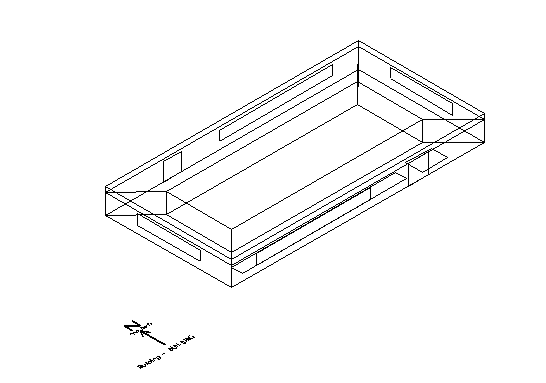
\includegraphics[width=0.9\textwidth, height=0.9\textheight, keepaspectratio=true]{media/image020.png}
\caption{Schematic for Exercise 2. \protect \label{fig:schematic-for-exercise-2.}}
\end{figure}

\subsection{Details of the Exercise}\label{details-of-the-exercise-000}

\subsubsection{Building Description}\label{building-description}

\begin{itemize}
\item
  Single floor rectangular building 30.5 m (100 ft) by 15.2 m (50 ft) by 3m (10 ft) high.
\item
  Building is oriented with the long axis running east-west.
\item
  Floor Area 463.6 m2 (5000 ft2).
\item
  5 occupied zones - 4 exterior, 1 interior, zone height 2.4 m (8 ft). Exterior zone depth is 3.7 m (12 ft).
\item
  1 plenum zone 0.6 m (2 ft) high.
\item
  Windows on all 4 facades
\item
  South and north facades have glass doors.
\item
  South facing glass is shaded by overhangs.
\item
  Walls are wood shingle over plywood, insulation, and gypsum board.
\item
  Roof is gravel built up roof with mineral board insulation and plywood sheathing.
\item
  Floor slab is 0.1 m (4 in) heavy concrete.
\item
  Windows and glass doors are double pane Low-e clear glass with argon gap.
\item
  Window to wall ratio is approximately 0.3.
\item
  Lighting is 16 W/m2 (1.5 W/ft2).
\item
  Office electric equipment is 10.8 W/m2 (1.0 W/ft2).
\item
  1 occupant per 9.3 m2 (100 ft2) of floor area.
\item
  Infiltration is 0.25 air changes per hour (always on, proportional to wind speed).
\item
  * Refers to specific glass type included in the EnergyPlus datasets directory
\item
  ~~~~~~~~~~~ (WindowGlassMaterials.idf)
\end{itemize}

\subsubsection{Space Conditioning}\label{space-conditioning}

\begin{itemize}
\item
  Heating setpoints:~~ 21.1C (70F) occupied, 12.8C (55F) unoccupied
\item
  Cooling setpoints:~~ 23.9C (75F) occupied, 40.0C (104F, system off) unoccupied
\item
  Plenum zone not controlled
\end{itemize}

\subsubsection{Environment}\label{environment}

\begin{itemize}
\item
  Location:~~~~~~~~~~~~~~~~~~ Chicago, Illinois, USA
\item
  Design Days:~~~~~~~~~~~~ Summer, Winter
\item
  Annual Simulation Period:~~~ Jan 1 -- Dec 31
\item
  Ground Temperatures:~~~~~~~~ from Slab preprocessor (20.4 to 23.0 C)
\end{itemize}
